\section*{Big-O intuition%
\TAGS{big-o}}

\begin{center}
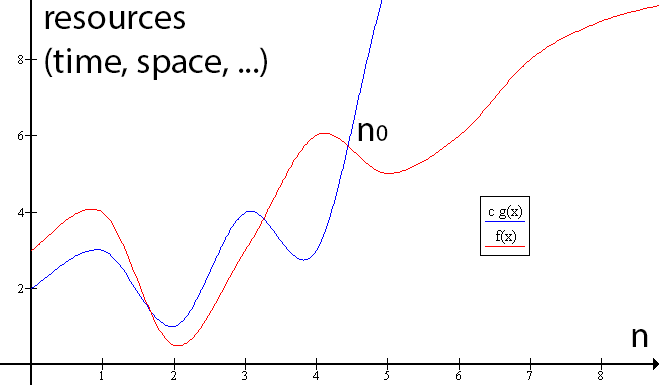
\includegraphics[width=0.5\textwidth]{\img/Big-O-notation.png}\\[0.5ex]
\emph{To the left of $n_0$, the functions can do anything.
\\To its right, $c \, g(n)$ is
always greater than or equal to $f(n)$.}
\end{center}

Intuitively, $O(g(n))$ is the set of all functions that $g(n)$ can
outpace in the long run (with the help of a constant scaling
factor). For example, $n^2$ eventually outpaces $3n\log(n)+5n$, so
$3n\log(n)+5n \in O(n^2)$. Because we only care about long run
behavior, we generally can discard constants and can consider only the
most significant term in a function.

There are actually
\emph{infinitely many functions}
that are in $O(g(n))$: If $f(n) \in O(g(n))$, then
$\frac{1}{2}f(n) \in O(g(n))$ and $\frac{1}{4}f(n) \in O(g(n))$ and $2 f(n) \in O(g(n))$.
In general, for any constants $k_1, k_2$, $k_1 f(n)+k_2 \in O(g(n))$.
